\documentclass[10pt,a4paper]{article}
\usepackage[utf8]{inputenc}
\usepackage{amsmath}
\usepackage{amsfonts}
\usepackage{amssymb}
\usepackage{color}
\usepackage{graphicx}
\usepackage{listings}
\author{K.M.J. Jacobs (s4134621) \and Zhuoran Liu (s4594851) \and Ankur Ankan (s4753828) \and Code file: Ising.m}
\title{Ising Model}

% Set all of these to false for the final document
\newif\ifrequirements
%\requirementstrue
\requirementsfalse

\begin{document}
\maketitle

\ifrequirements
\color{red}
\textbf{Document requirements shown by flag \texttt{requirementstrue}.}
\textbf{Set flag \texttt{requirementsfalse}.}

\color{blue}
\section{Guidelines for ML assignments}
Note: All reports should be handed in before the end of January 2017. Hard deadline is \textbf{January 31 at 23.59}. Any questions about the below points please contact me (Hans-Christian Ruiz). For the assignments please refer to the ML course page.

\subsection{Requirements to hand in the reports}
\begin{itemize}
\item Hand in each report as a SINGLE document with all figures, code, etc (other "extra" files will not be considered). Hand in printed in my post box (Ruiz, wing 8, ground floor).
\item In addition, hand in the code that can be run stand-alone. Send us an email with a zip-file containing the codes for all assignments. The zip-file should be named with the last names of all group members. Each code in the zip-file should be named as AssignmentName where AssignmentName is: Ising, BM, MNIST, Lasso, Control
\item Your name on each report and the name of the corresponding code file in the zip-file that you sent us via email.
\item The report should be well structured and clear.
\item Figures need to have a caption explaining in detail what they show. 6. No more than 8 pages (excluding references and code) with 12 pts font.
\end{itemize}

\subsection{Minimal requirements of the content}
The report for each exercise addresses following points:
\begin{itemize}
\item Introduction: summarizes the underlying theory and algorithm(s). It should be a short description of the theoretical background and expla- nation of the method considered (no more than a page!).
\item Problem statement: Itemizes a number of research questions that you address
\item Results: Detailed description of the different numerical studies that you have performed with plots and specification of the parameter settings (a) Precise, clear description of what you have done, with the used formulas and the argumentation of why you have done it; e.g. what measure of convergence you used, are there alternatives? (b) Figures with a detailed explanation of what the relevant results are (c) An analysis of the results (for example: is the result as expected? why?/why not? what does the result mean? etc...)
\item General discussion/Conclusions: A summary of the main findings and conclusions (no more than half page!)
\item Appendix: If the exercise requires to write a code, add the code in the appendix. The code should have the following characteristics (a) Well documented, comments! (b) Suitable structure for readability, e.g. indentation, proper (mnemonic) variable naming. 6. Note: The code will not be evaluated based on whether it is optimized or not, only if it is clearly readable. But, IT MUST RUN STAND- ALONE!
\end{itemize}

\color{black}
\fi

\newpage
\tableofcontents

\newpage
\section{Introduction}
This work is mainly about the simulated annealing process. There are two parts in total. The first part mainly considered the iterative improvement. For both ferro-magnetic and frustrated situations, we will choose to flip $1$, $2$ or more spins to make the cost lower than before. The algorithm terminates when no improvement for any state.


\section{Problem statement}
In the first part of the assignment, we are asked to investigate in the given iterative method for both the ferromagnetic and a frustrated system.
For the second part of the assignment, both the iterative method and simulated annealing are compared on different problems.

The research questions are the following:
\begin{enumerate}
\item How does Simulated Annealing improve upon the Iterative method?
\item What is the influence of different parameter settings on Simulated Annealing?
\end{enumerate}

\section{Results}
\subsection{Exercise 1.1}
Firstly, we did some experiments in the ferro-magnetic situation with $n=100$. Firstly, in the situation neighbourhood size is $1$, we need $436$ restarts to get the minimal energy $-2512$. When we changed the neighbourhood size to $2$, it just need $207$ restarts.\\
Then, we did some experiments in the frustrated situation with $n=100$. When neighbourhood size is $1$, we did $1.000.000$ restarts found minimal energy is $-602$. Then we did with neighbourhood size $2$, and found minimal energy is $-736$ with $1.000.000$ restarts. So for the frustrated situation, it is not easy to convergence. Especially with less neighbourhood size.
\subsection{Exercise 1.2}
In frustrated situation, it is not easy to get the minimal energy.
We firstly did experiments with restart number $100000$, it will take on average $10$ seconds. The minimal energy is more or less $-736$, but we got it ranges from $-736$ to $-586$ in $5$ times experiments.\\
Then we changes the restart number to $1.000.000$. It costed $95$ seconds, and got results ranged from $-704$ to $-644$ . It ranges less, but also didn't yield nice results.\\
When increase the restarts to $10.000.000$, it will take $998$ seconds and still didn't give a good result.

\subsection{Exercise 2.1}
\subsubsection{Plot reconstruction for $n=50$}
\begin{figure}[h]
\centering
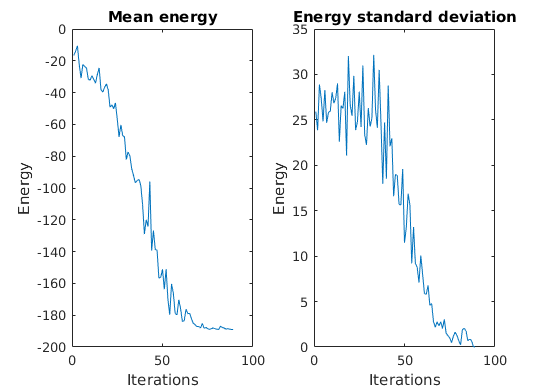
\includegraphics[scale=0.6]{../sa/sa_frustrated.png}
\caption{Simulated Annealing in which $1000$ samples are generated at each temperature using Metropolis-Hasting with $\beta_0=\frac{1}{\max(dE)}$ and $\beta_{t+1} = \beta_t \cdot 1.05$ for a frustrated system with $n=50$.}
\label{fig:sa_frustrated}
\end{figure}

\begin{figure}[h]
\centering
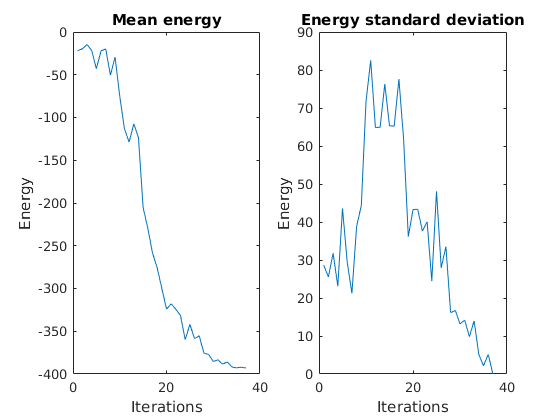
\includegraphics[scale=0.6]{../sa/sa_ferromagnetic.png}
\caption{Simulated Annealing in which $1000$ samples are generated at each temperature using Metropolis-Hasting with $\beta_0=\frac{1}{\max(dE)}$ and $\beta_{t+1} = \beta_t \cdot 1.05$ for a ferromagnetic system with $n=50$.}
\label{fig:sa_ferromagnetic}
\end{figure}

In figure \ref{fig:sa_frustrated}, the resulting plots are shown when simulated annealing is applied on a problem with $n=50$ in the case that the system is frustrated.

In figure \ref{fig:sa_ferromagnetic}, the resulting plots are shown when simulated annealing is applied on a problem with $n=50$ in the case that the system is ferromagnetic.

\subsubsection{Choice of $\beta$ and \texttt{factor}}

\begin{align}
p(x) = \frac{\exp(-\beta E(x))}{Z}
\label{eq:sa_p}
\end{align}

In equation \ref{eq:sa_p}, the definition of the probability distribution of a state $x$ is shown. If you take $\beta \rightarrow \infty$, then $p(x) \rightarrow 0$ and all states are assigned approximately equal probability. By that, the sampling procedure can get stuck in any state if there are no neighbours with higher probability. Since the probabilities are approximately equal, it is very hard to find any better neighbours. When we ran an experiment with $\beta \approx 1000$ we found indeed that there were only a few number of iterations ($< 10$) which is caused by the fact that it gets stuck in a particular state. Also, the probability that the final state is a global optimum is extremely low.

The lower the choice for $\beta$, the more samples are accepted during the sampling procedure. This will result in a better final state and a better approximation for the minimum energy. Because more samples are accepted, it will take a longer time to finish the simulation.

In conclusion, smaller $beta$ ($beta \rightarrow 0$) will result in better results but it takes a longer time to finish the simulation.

The \texttt{factor} variable defines how $\beta$ is increased at each timestep (since $\beta_{t + 1} = \beta_t \cdot \texttt{factor}$). The more $\texttt{factor} \rightarrow 1$, the more slowly $\beta$ grows and therefore the more time it takes for the sampling procedure. The larger $\texttt{factor}$, the less time it takes, but the results get worse.

\subsubsection{Influence of the length of the Markov Chain}
The first few samples of a Markov Chain are samples in which the system is explored. The probability of accepting any other state is relatively high. Therefore, the mean energy of these samples fluctuates a lot. If more samples are taken from the Markov Chain, the probability of accepting other states decreases. Therefore, the mean energy of the tail of the Markov Chain is stable. The longer the chain is, the longer the tail of the chain is and therefore the more stable the mean energy becomes. If the chain is shorter, then the mean energy will fluctuate more.

\newpage
\subsubsection{Influence of $\beta$, \texttt{factor} and the length of the Markov Chain on the minimum energy}

\begin{table}[h]
\centering
\begin{tabular}{|lll|rr|}
\hline
$\mathbf{\beta}$ & \texttt{factor} & $T_1$ & $\mathbb{E}(E_{\min})$ & $Var(E_{\min})$\\
\hline
0.01 & 1.01 & 10 & -127 & 1774\\
0.01 & 1.01 & 1000 & -196 & 3\\
0.01 & 1.05 & 10 & -145 & 264\\
\textbf{0.01} & \textbf{1.05} & \textbf{1000} & \textbf{-197} & \textbf{0}\\
0.01 & 2.00 & 10 & -190 & 47\\
\textbf{0.01} & \textbf{2.00} & \textbf{1000} & \textbf{-197} & \textbf{0}\\
2 & 1.01 & 10 & -112 & 798\\
2 & 1.01 & 1000 & -191 & 43\\
2 & 1.05 & 10 & -114 & 141\\
2 & 1.05 & 1000 & -181 & 260\\
2 & 2.00 & 10 & -106 & 1309\\
2 & 2.00 & 1000 & -187 & 53\\
\hline
\end{tabular}
\caption{The influence in the frustrated case of different configurations on the found minimum energy. $\mathbb{E}$ is the mean of the found minimum energies and $Var(E)$ is the variance of the found minimum energies. $T_1$ is the number of samples used for the Metropolis-Hasting algorithm. The results are based on $5$ runs of the algorithm. In the rows which have a bold typeface, the minimum of the problem was found.}
\label{tab:parameters_frustrated}
\end{table}

\begin{table}[h]
\centering
\begin{tabular}{|lll|rr|}
\hline
$\mathbf{\beta}$ & \texttt{factor} & $T_1$ & $\mathbb{E}(E_{\min})$ & $Var(E_{\min})$\\
\hline
0.01 & 1.01 & 10 & -255 & 7438\\
\textbf{0.01} & \textbf{1.01} & \textbf{1000} & \textbf{-408} & \textbf{0}\\
0.01 & 1.05 & 10 & -260 & 7947\\
\textbf{0.01} & \textbf{1.05} & \textbf{1000} & \textbf{-408} & \textbf{0}\\
\textbf{0.01} & \textbf{2.00} & \textbf{10} & \textbf{-408} & \textbf{0}\\
\textbf{0.01} & \textbf{2.00} & \textbf{1000} & \textbf{-408} & \textbf{0}\\
\textbf{2} & \textbf{1.01} & \textbf{10} & \textbf{-408} & \textbf{0}\\
\textbf{2} & \textbf{1.01} & \textbf{1000} & \textbf{-408} & \textbf{0}\\
\textbf{2} & \textbf{1.05} & \textbf{10} & \textbf{-408} & \textbf{0}\\
\textbf{2} & \textbf{1.05} & \textbf{1000} & \textbf{-408} & \textbf{0}\\
\textbf{2} & \textbf{2.00} & \textbf{10} & \textbf{-408} & \textbf{0}\\
\textbf{2} & \textbf{2.00} & \textbf{1000} & \textbf{-408} & \textbf{0}\\
\hline
\end{tabular}
\caption{The influence in the ferromagnetic case of different configurations on the found minimum energy. $\mathbb{E}$ is the mean of the found minimum energies and $Var(E)$ is the variance of the found minimum energies. $T_1$ is the number of samples used for the Metropolis-Hasting algorithm. The results are based on $5$ runs of the algorithm. In the rows which have a bold typeface, the minimum of the problem was found.}
\label{tab:parameters_ferromagnetic}
\end{table}

In table \ref{tab:parameters_frustrated} and \ref{tab:parameters_ferromagnetic} a comparison is made between different configurations and the found optimal energy. It indeed corresponds to our findings that a larger $T_1$ yields better results. Also, the more $\beta \rightarrow 0$ and $\texttt{factor} \rightarrow 1$, the better the results will get.

For the ferromagnetic problem, we get that $E_{\min} \approx -408$ and for the frustrated problem we found that $E_{\min} \approx -197$. As we explain later, different runs for $\texttt{makedata}$ when using the same random number generator seed resulted in different values of $w$. Therefore, we keep $w$ fixed in both situations.

\subsubsection{Comparison between Simulated Annealing (SA) and the iterative method (Iter)}

\textbf{Ferromagnetic system}\\
For a ferromagnetic system, both Simulated Annealing and the iterative method will converge.

For the iterative method, the running time depends on the number of restarts as specified in the iterative method.

The running time of the Simulated Annealing depends on the number of samples for estimating the maximum $dE$ and it depends on the length of the Markov Chain.

For the iterative method with a neighbourhood size of $2$ and $800$ number of restarts and with a dimensionality $n=250$ we reach approximately the fastest running time of $0.29$ seconds.

For the Simulated Annealing, we reached approximately the fastest running time of $0.88$ seconds with $n=250$, a Markov Chain length of $1000$ and the number of samples for estimating $\max(dE)$ equal to $100$.

\textbf{Frustrated system}\\
For the iterative method with a neighbourhood size of $2$ and $150.000$ number of restarts and with a dimensionality $n=250$ we reach approximately the fastest running time of $58$ seconds.

For the Simulated Annealing, we reached approximately the fastest running time of $13$ seconds with $n=250$, a Markov Chain length of $1000$ and the number of samples for estimating $\max(dE)$ equal to $100$.

\textbf{Conclusion}\\
Since there are so many parameters, it is hard to compare both methods. Also the running time depends on the hardware which is used and even if we analyze the running time by means of upper bounds, there are some random variables which cause undeterministic running times.

If the running times are compared when solving a frustrated system, then it is extremely difficult for the iterative method to find the optimal solution. The Simulated Annealing however is faster and finds the optimal solution.

\subsubsection{Comparison for $n=200$}
We had difficulties in comparing $w$ since the $\texttt{sprandsym}$ gave different values even if the seed for the random number generator was set to the same number on different computers. Therefore, we computed a random symmetric binary matrix $w$ in ourselves. This yields the same $w$ matrix on different computers when we used the same number for the seed for the random number generator.

On both computers, we found $E_{\min} = -10080$.

\section{Discussion and Conclusions}

\subsection{How does Simulated Annealing improve upon the Iterative method?}
The iterative method does get stuck in local minima easily. So in the case of a frustrated system when there are many local minima, the iterative method will not find a global solution to the problem. Simulated Annealing does find a global optimum to these problems.

The running time of the iterative method and Simulated Annealing are hard to compare. For easy problems, the running time of the iterative method is approximately equal to the running time of Simulated Annealing. For hard problems, the iterative method will not converge at all for most of the problems whereas Simulated Annealing will find a solution quite fast.

\subsection{What is the influence of different parameter settings on Simulated Annealing?}
For simple problems like in the ferromagnetic case, almost any configuration of parameters will work.

For harder problems like the frustrated system with large $n$, parameters $\beta \rightarrow 0$ and $\beta > 0$ and a $\texttt{factor}$ close and strictly larger than $1$ and $T_1 \rightarrow \infty$ are giving good results.

\newpage
\section{Appendix}

\subsection{Generation of a binary symmetric random matrix}
\begin{lstlisting}[language=Matlab]
rand('state',0)
n=50;
p=n;
w=sprandsym(n,p);
%w=(w>0)-(w<0); % this choice defines a frustrated system
w=(w>0); % this choice defines a ferro-magnetic (easy) system
w=w-diag(diag(w));
\end{lstlisting}

\subsection{Both the iterative method and Simulated Annealing}
\begin{lstlisting}[language=Matlab]
% problem definition
% minimize E= 0.5 x^T w x, with x=x_1,...,x_n and x_i=0,1
% w is a symmetric real n x n matrix with zero diagonal

METHOD='sa';
NEIGHBORHOODSIZE=1;
n_restart =100;

switch METHOD,
case 'iter'

	E_min = 10000;
    x = 2*(rand(1,n)>0.5)-1;
	for t=1:n_restart,

		% initialize
		E1 = E(x,w);
		flag = 1;
	
		while flag == 1,
			flag = 0;
			switch NEIGHBORHOODSIZE,
			case 1,
				% choose new x by flipping one bit i
				% compute dE directly instead of subtracting E's of
				% different states because of efficiency
                bit = randi([1, numel(x)]);
                x_new = x;
                x_new(bit) = x_new(bit) * -1;
                E2 = E(x_new,w);
                % Check whether the new energy is smaller than the old
                % energy and update the 'best' state
                if E2 < E1
                    x = x_new;
                    E1 = E2;
                    flag = 1;
                    break;
                end
			case 2,
				% choose new x by flipping bits i,j
                bit1 = randi([1, numel(x)]);
                bit2 = randi([1, numel(x)]);
                while bit2 == bit1
                    bit2 = randi([1, numel(x)]);
                end
                % Make 3 states and check whether the energy decreases
                x_new1 = x;
                x_new2 = x;
                x_new3 = x;
                x_new1(bit1) = x_new1(bit1) * -1;
                x_new2(bit2) = x_new2(bit2) * -1;
                x_new3(bit1) = x_new3(bit1) * -1;
                x_new3(bit2) = x_new3(bit2) * -1;
                E_new1 = E(x_new1,w);
                E_new2 = E(x_new2,w);
                E_new3 = E(x_new3,w);
                
                % Check if the energy of the state in which the first bit
                % is flipped is the best neighbour in terms of energy
                if E_new1 < E1 & E_new1 < E_new2 & E_new1 < E_new3
                    x = x_new1;
                    E1 = E_new1;
                    flag = 1;
                end
                
                % Check if the energy of the state in which the second bit
                % is flipped is the best neighbour in terms of energy
                if E_new2 < E1 & E_new2 < E_new1 & E_new2 < E_new3
                    x = x_new2;
                    E1 = E_new2;
                    flag = 1;
                    break;
                end
                
                % Check if the energy of the state in which both bits are
                % flipped is the best neighbour in terms of energy
                if E_new3 < E1 & E_new3 < E_new1 & E_new3 < E_new2
                    x = x_new3;
                    E1 = E_new3;
                    flag = 1;
                    break;
                end
            end;
		end;
		E_min = min(E_min,E1);
	end;
	E_min
case 'sa'
	% initialize
	x = 2*(rand(1,n)>0.5)-1;
	E1 = E(x,w);
	E_outer=zeros(1,100);	%stores mean energy at each temperature
	E_bar=zeros(1,100);		% stores std energy at each temperature

	% initialize temperature
	max_dE=0;
    x_old = x;
    
    % Estimate the maximum change of energy by taking random samples and
    % take one random neighbour and compare the energies
	switch NEIGHBORHOODSIZE,
        case 1,
			% estimate maximum dE in single spin flip
            for round = 1:10000
                x_1 = 2*(rand(1,n)>0.5)-1;
                bit = randi(1, n);
                x_2 = x_1;
                x_2(bit) = x_2(bit) * -1;
                dE = E(x_2, w) - E(x_1, w);
                max_dE = max(max_dE, dE);
            end
        case 2,
			% estimate maximum dE in pair spin flip
        end;
        
	beta_init=1/max_dE;	% sets initial temperature
    
    %beta_init = 0.1;
    
	T1=1000; % length markov chain at fixed temperature
	factor=1.05 ; % increment of beta at each new chain
    
    beta_init = 2;
    factor = 2;
    T_1=1000;
    
	beta=beta_init;
	E_bar(1)=1;
	t2=0;
	while t2 == 0 | E_bar(t2) > 0,
        t2=t2+1;
		beta=beta*factor;
		E_all=zeros(1,T1);
		for t1=1:T1,
			switch NEIGHBORHOODSIZE,
			case 1,
				% choose new x by flipping one random bit i
				% perform Metropolis Hasting step
                bit = randi(n, 1);
                x_new = x;
                x_new(bit) = x_new(bit) * -1;
                E2 = E(x_new,w);
                dE = E2 - E1;
                a = exp(-dE * beta);
                a = min(1, a);
                if a > rand()
                    x = x_new;
                    E1 = E2;
                end
                E_all(1,t1) = E1;
			case 2,
				% choose new x by flipping random bits i,j
				% perform Metropolis Hasting step
                bit1 = randi(n, 1);
                bit2 = bit1;
                
                % Choose a second bit which is unequal to the first bit
                while bit2 == bit1
                    bit2 = randi(n, 1);
                end
                
                % Compute the proposed states
                x_new = x;
                x_new(bit1) = x_new(bit1) * -1;
                x_new(bit2) = x_new(bit2) * -1;
                
                % First check for the state in which both bits are flipped
                E2 = E(x_new, w);
                dE = E2 - E1;
                a = exp(-dE * beta);
                a = min(1, a);
                if a > rand()
                    x = x_new;
                    E1 = E2;
                else
                    % Then check for the state in which only the first bit is
                    % flipped
                    x_new = x;
                    x_new(bit1) = x_new(bit1) * -1;
                    E2 = E(x_new, w);
                    dE = E2 - E1;
                    a = exp(-dE * beta);
                    a = min(1, a);
                    if a > rand()
                        x = x_new;
                        E1 = E2;
                    else
                        % Finally check for the state in which only the
                        % second bit is flipped
                        x_new = x;
                        x_new(bit1) = x_new(bit1) * -1;
                        E2 = E(x_new, w);
                        dE = E2 - E1;
                        a = exp(-dE * beta);
                        a = min(1, a);
                        if a > rand()
                            x = x_new;
                            E1 = E2;
                        end
                    end
                end
                E_all(1,t1) = E1;
			end;
			% E1 is energy of new state
			E_all(t1)=E1;
		end;
		E_outer(t2)=mean(E_all);
		E_bar(t2)=std(E_all);
		[t2 beta E_outer(t2) E_bar(t2)] % observe convergence
	end;
	E_min=E_all(1) % minimal energy 
end;

subplot(1, 2, 1);
plot(1:t2,E_outer(1:t2))
xlabel('Iterations');
ylabel('Energy');
title('Mean energy');

subplot(1, 2, 2);
plot(1:t2,E_bar(1:t2))
xlabel('Iterations');
ylabel('Energy');
title('Energy standard deviation');
\end{lstlisting}
\end{document}